%% Marco Teórico C1 %%

\chapter{Paradigmas}

``Las herramientas que utilizamos tienen una profunda (¡y retorcida!) influencia en nuestros hábitos de pensamiento, y, por lo tanto, en nuestra habilidad mental'', Edsger Dijkstra. \\

Los paradigmas de programación guían la forma en que debe construirse una solución para resolver problemas utilizando herramientas computacionales. Cada paradigma tiene sus ventajas y desventajas de acuerdo al tipo de problema que se deseé resolver. En este capítulo se revisan las dos principales corriente \emph{imperativa} y \emph{funcional}, soportadas en las \emph{Máquinas de Turing} y el \emph{Cálculo Lambda}, respectivamente.

\section{Modelo computacional}

Para el estudio de la \emph{computación} desde un enfoque teórico, es necesario utilizar abstracciones que cumplan con las siguientes restricciones:

\begin{enumerate}
	\item El modelo debe ser lo suficientemente poderoso para poder realizar cualquier método computacional físicamente realizable. Sólo de esta forma se puede garantizar que los resultados encontrados puedan ser aplicados en cualquier \emph{Computador Universal} (aquellos que pueden realizar todos las operaciones conocidas sobre una entrada discreta).
	\item El modelo debe ser lo suficientemente simple para facilitar los análisis y las demostraciones a realizar, siendo menester que dicha abstracción elimine detalles innecesarios, cómo por ejemplo, las especificaciones propias de la máquina o las restricciones de un lenguaje de programación específico.
\end{enumerate}  

En ese órden de ideas, han surgido múltiples abstracciones que si bien, han inspirado caminos diferentes para la solución de problemas, han resultado siendo equivalentes en poder computacional; es decir, que en los modelos que se exponen a continuación, aplican los mismos principios de la \emph{teoría computacional}, así como también tienen los mismos límites en cuánto a \emph{computabilidad} se refiere.

\subsection{Máquina de Turing}

``(Turing)ha tenido éxito por primera vez en encontrar una definición absoluta de una interesante noción epistemológica, por ejemplo, una que no depende del formalismo seleccionado'', Kurt Gödel. \\

La Máquina de Turing (TM, por sus siglas en inglés), desarrollada por el matemático Alan Turing, ha servido como el principal modelo bajo el cuál se han construido las computadoras modernas.

\begin{defn}[Definición formal de una TM]\end{defn}

Formalmente, una TM $M$ está descrita por una tupla $(\Gamma, Q, \delta)$  \cite{Arora2009}, que contiene:

\begin{itemize}
\item Un conjunto finito $\Gamma$ de símbolos que las cintas de $M$ pueden contener. Usualmente se tienen 3 cintas, una de entrada, una de trabajo y una de salida, y sobre estas la máquina realiza las operaciones necesarias. Se asume que $\Gamma$ tiene un símbolo ``blank'', denotado por $\Box$; un símbolo ``start'', denotado por $\rhd$; y los número 0 y 1|. Llamamos $\Gamma$ el \emph{alfabeto} de $M$.

\item Un conjunto finito $Q$ de los posibles estados en los que el registro de $M$ puede encontrarse. Asumimos que $Q$ contiene designado un estado inicial, denotado por $q_{start}$, y un estado de terminación (\emph{halting}), denotado por $q_{halt}$.

\item Una función $\delta$: $Q \times \Gamma^k \to Q \times \Gamma^{k-1} \times \{L,S,R\}^k$, donde $k \geq 2$ y $L$: left. $S$: stay. $R$: right., describiendo las reglas que $M$ usa para realizar cada paso. Esta función es llamada \emph{función de transición} de $M$. 
\end{itemize}

Una máquina de Turing es un computador moderno simplificado. Cualquier algoritmo puede traducirse en un conjunto de reglas y símbolos, de forma que pueda ser simulado por una TM.

\begin{figure}
	\centering
	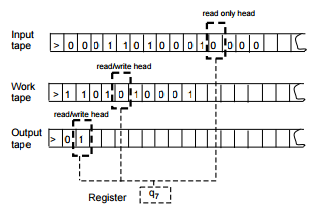
\includegraphics{images/tm}
	\caption{TM con 3 cintas.}
\end{figure}

\subsection{Cálculo Lambda}

El cálculo lambda $\Lambda$ desarrollado por Alonso Church en los 30 para dar una teoría general de las funciones. Tiene por objeto formalizar el empleo de funciones como transformación de argumentos en resultados empleando 
un conjunto de axiomas, y reglas de inferencia.

\subsubsection{Sintaxis}

Dado un conjunto \texttt{A} de nombres de variables tal que $\vert$ 
\texttt{A} $\vert = \mathbb{N}$, una expresión lambda \texttt{<expr>} es una produccion de FNB ``Forma normal de Backus $\mathfrak{F}$":

\begin{verbatim}
<expr> ::= <variable> 
        |  <variable>.<expr> 
        |  (<expr><expr>)
\end{verbatim}

\begin{note}
Para denotar términos usamos letras mayúsculas \texttt{M,N, $\dots$} y para denotar variables letras  minúsculas \texttt{$x,y, \dots$}
\end{note}

Una abstracción funcional crea procedimientos y funciones y los invocara mediante un nombre donde se destaca qué hace la función y se ignora cómo lo hace, está será:

\texttt{$\lambda$<variable>.<expr>}
donde:
\texttt{$\lambda$<variable>} es la lista de argumentos
\texttt{<expr>} es el contenido de la abstracción funcional

Una función con más de un argumento se representará:
\texttt{$\lambda $x$_1. $x$_2. \dots $x$_n. $M}

\begin{defn}[Equivalencia entre expresiones de $\Lambda$]\end{defn}

Aplicación funcional  \texttt{(M N)} la cual produce un resultado \texttt{R} la consistencia implica una interpretacion equivalente,
es decir \texttt{(M N)} $\equiv$ \texttt{R}, luego representan lo mismo.
El resultado de una aplicación funcional será obtenido mediante la generación de expresiones equivalentes:

\begin{defn}[Relaciones de equivalencia entre expresiones de $\Lambda$]
\end{defn}
\begin{itemize}
\item Reflexividad: \texttt{M $\equiv$ M}
\item Simetría: \texttt{M $\equiv$ N $\Rightarrow$ N $\equiv$ M}
\item Transitividad: \texttt{M $\equiv$ N $\wedge$ N $\equiv$ P $\Rightarrow$  M $\equiv$ P}
\item \texttt{M $\equiv$ N $\Rightarrow$ (M P) $\equiv$ (N P)}
\item \texttt{M $\equiv$ N $\Rightarrow$ (P M) $\equiv$ (P N)}
\item \texttt{M $\equiv$ N $\Rightarrow$ $\lambda$x.N $\equiv$ $\lambda$x.M}
\end{itemize}

\begin{defn}[Ocurrencia $\succ$ de un $\lambda$-termino]\end{defn}
\begin{itemize}
\item \texttt{$\succ$P $\in$ P}
\item \texttt{$\succ$P $\in$ M $\vee$ N $\Rightarrow \ \succ$P $\in$ (M N)}
\item \texttt{$\succ$P $\in$ M $\vee$ P $\equiv$ x $\Rightarrow \ \succ$P $\in$ ($\lambda$x.M)}
\end{itemize}

\begin{defn}[Ocurrencia $\succ$ de un $\lambda$-variable ligada \texttt{b} o libre \texttt{f}]\end{defn}
Una ocurrencia de la variable \texttt{b} en un término \texttt{P} es ligada sí y solo sí, \texttt{b} ocurre en un subtérmino de \texttt{P} de la forma \texttt{$\lambda$b.M} es decir 
\texttt{Q $\subset $ P $ := \lambda$b.M
$\Rightarrow \ \succ$b $\in$ P $\Leftrightarrow$ 
$\succ$x $\in$ Q}. \\
La ocurrencia es libre cuando \\
\texttt{$\succ$f $\in$ N $ := \lambda$z.M $\wedge$
f$\neq$z 
$\Rightarrow \ \succ$f $\in$ N $\Leftrightarrow  
$ f $\equiv$ N $\vee \ \succ$f $\in$ M }

\begin{note}
Llamamos $\mathit{f}$ el conjunto de variables libres
y $\mathit{b}$ el de ligadas, denotando por \texttt{f} y \texttt{b} sus elementos
\end{note}

\begin{defn}[$\alpha-$equivalencia $\equiv_{\alpha}$]\end{defn}

\texttt{$\succ$x $\in$ M $\Rightarrow$ ($\lambda$b.M)[x/y] $\equiv_{\alpha} \lambda$b.N}

\begin{defn}[$\beta$-reducción $\rightarrow_{\beta}$]\end{defn}
\texttt{($\lambda$f.M N) $\equiv$ [N/f] M} donde
\texttt{[N/f] M} se obtiene de introducir \texttt{N} y no \texttt{f} si \texttt{$\succ$f $\in$ M}

\begin{defn}[$\alpha$-conversion $\rightarrow_{\alpha}$]\end{defn}
\texttt{($\lambda$b.M) $\rightarrow_{\alpha}$ ($\lambda$b.N)}
 
\begin{note}
La $\alpha$-conversion no es posible si la equivalencia resultante genera nuevas variables ligadas que cambien el sentido a la abstraccion original.
\end{note}

\begin{defn}[$\eta$-conversion $\rightarrow_{\eta}$]\end{defn}
\texttt{$\succ b \in M \Rightarrow$ ($\lambda$b.Mb) $\rightarrow_{\eta}$ M}
\begin{note}
Genera conversiones sobre funciones, es la aproximacion funcional de la extensionalidad de conjuntos.
\end{note}

\section{Lenguajes de programación}

\subsection{Imperativo}

\subsection{Declarativo}